% !TeX document-id = {a4f138bc-afad-4341-8d0d-d3abfb861561}
%%%%%%%%%%%% Attribution %%%%%%%%%%%%
% This template was created by 
% Chuck F. Rocca at WCSU and may be
% copied and used freely for 
% non-commercial purposes.
% 10-17-2021
%%%%%%%%%%%%%%%%%%%%%%%%%%%%%%%%%%%%%

%%%%%%% Start Document Header %%%%%%%
% In creating a new document
% copy and paste the header 
% as is.
%%%%%%%%%%%%%%%%%%%%%%%%%%%%%%%%%%%%%


\documentclass{article}

%%%% Header Information %%%%
    %%% Document Settings %%%%
    \usepackage[utf8]{inputenc}
    \usepackage[
        twoside,
        top=1in,
        bottom=0.75in,
        inner=0.5in,
        outer=0.5in
    ]{geometry}
    \pagestyle{myheadings}

%%%% Additional Commands to Load %%%%
    \usepackage{tcolorbox}
    \tcbuselibrary{skins}
    \usepackage{minted}
    \usepackage{color}
    \usepackage{tikz}
    \usetikzlibrary{calc}
    \usepackage{tabularx,colortbl}
    \usepackage{amsfonts,amsmath,amssymb}
    \usepackage{titling}
    \usepackage{mathrsfs}
    \usepackage{calc}
    \usepackage{xepersian}

%%%% Commands to Define Homework Boxes %%%%
%%%% Box Definition %%%%
    \newtcolorbox{prob}[1]{
    % Set box style
        sidebyside,
        sidebyside align=bottom,
    % Dimensions and layout
        width=\textwidth,
        toptitle=2.5pt,
        bottomtitle=2.5pt,
        righthand width=0\textwidth,
    % Coloring
        colbacktitle=gray!30,
        coltitle=black,
        colback=white,
        colframe=white,
    % Title formatting
        title={
            #1 \hfill نمره:\phantom{WWWW}
        },
        fonttitle=\large\bfseries
    }

%%%% Environment Definition %%%%
    \newenvironment{problem}[1]{
        \begin{prob}{#1}
    }
    {
        \tcblower
        \centering
        \vspace{\baselineskip}
        \end{prob}
    }



%%%% Document Information %%%%
    \title{\lr{HW1 Solutions}}
    \date{}
    \author{نویسنده : رضا شهریاری}

%%%%%%% End Document Header %%%%%%%


%%%% Begin Document %%%%
% note that the document starts with
% \begin{document} and ends with
% \end{document}
%%%%%%%%%%%%%%%%%%%%%%%%
\settextfont{BNAZANIN.TTF}

\begin{document}

%%%% Format Running Header %%%%%
\markboth{\theauthor}{\thetitle}

%%%% Insert the Title Information %%%
\maketitle


%%%% General Description of the Document %%%%


\raggedleft
%%%% Introduction to the General Template %%%%
\section{بخش مقدماتی (35 نمره)}
\centering


    \begin{problem}{سوال اول}
    	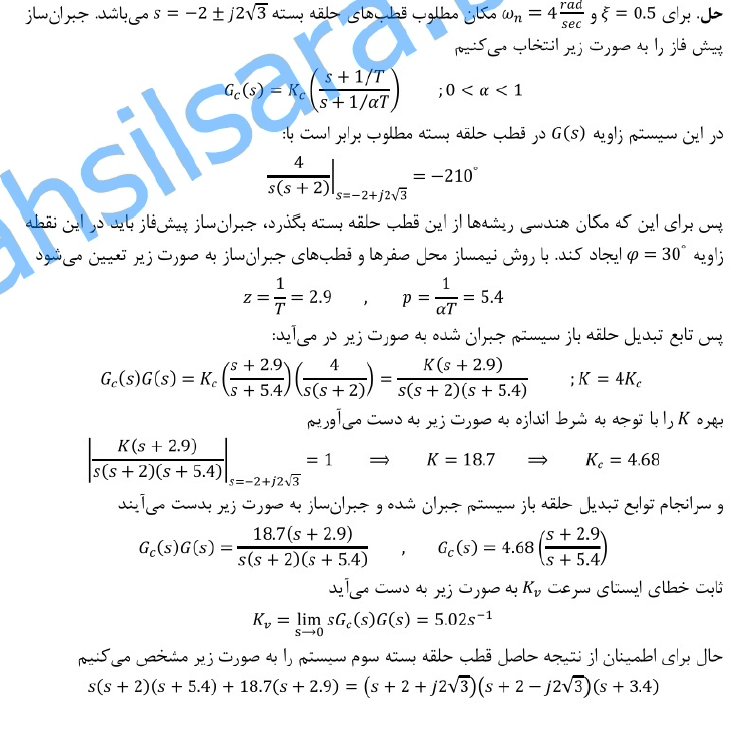
\includegraphics[width=\linewidth]{Resources/1.png}
   
    \end{problem}

    \begin{problem}{سوال دوم}
    	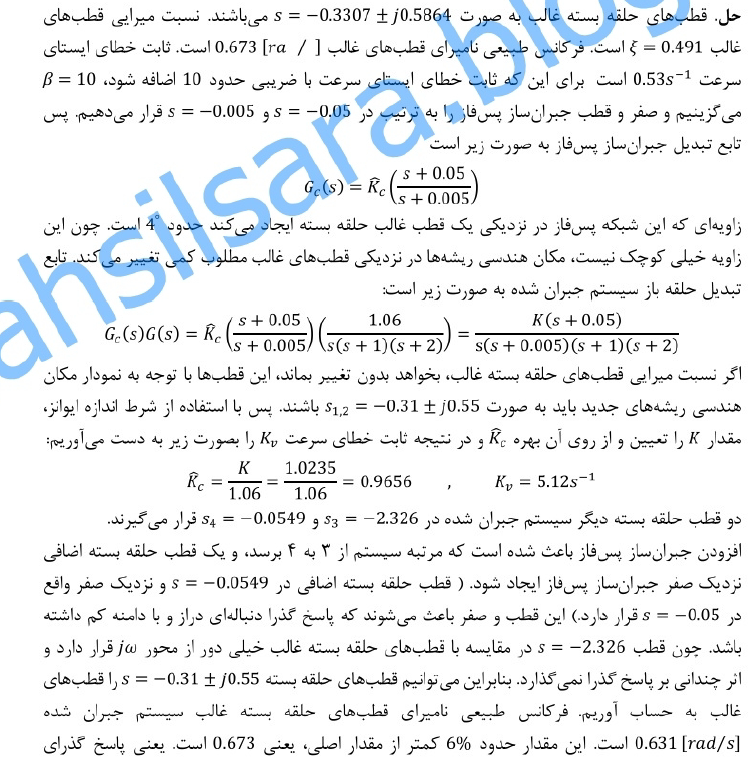
\includegraphics[width=\linewidth]{Resources/2.png}
    	
\includegraphics[width=\linewidth]{Resources/2-2.png}
    	
    \end{problem}
    
    \begin{problem}{سوال سوم}
    	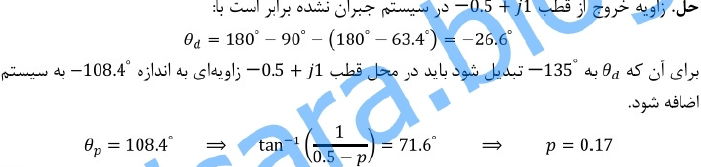
\includegraphics[width=\linewidth]{Resources/3.png}
    
    \end{problem}
    
    
    \begin{problem}{سوال چهارم}
        ایتدا حاشیه بهره و فاز را محاسبه می‌کنیم.
        فرکانسی که حاشیه بهره در آن اتفاق می‌افتد از رابطه زیر محاسبه می‌گردد.
        
        $-\pi/2 = \tan^{-1}(\omega/4) - \tan^{-1}(\omega/16)$
        
        این تساوی در 
        $\omega = 8$
        اتفاق می‌افتد.
        
        گین در فرکانس برابر
         $-1.94$
          دسی بل می‌باشد.
        
        جال حاشیه فاز این تابع تبدیل با بررسی فاز آن در 0 دسی بل بررسی کنید. حاشیه فاز -5.02 درجه می‌باشد.
        
        جبرانساز این سیستم باید به اندازه
        $15 + 5.02$
        درجه به فاز سیستم اضافه کند و همچنین
        $1.5+1.94$
        دسی بل به گین سیستم بیافزاید. 
        
        یک کنترلر \lr{PD} با تابع تیدیل زیر طراحی می‌کنیم
        
        $C = K(s+z)$
        
        باید در فرکانس 8.93، 20 درجه فاز تزریق شود و گین نیز باید در فرکانس 8 درجه 3.04 تزریق شود.
        
        $C = 2.2(s+4)$

    \end{problem}

    
    \begin{problem}{سوال پنجم}
    	سیستم حلقه باز جبران شده به صورت زیر است:
    	
    	\raggedleft
    	$C(s)G(s) = \frac{K}{s(0.5s+1)} (\frac{s}{z} + 1)$
    	
    	\raggedright
    	ثابت خطای سرعت استاتیکی به فرم زیر قابل محاسبه است:
    	
    	\raggedleft
    	${{K}_{v}}=\underset{s\to 0}{\mathop{\lim }}\,sC(s)G(s)=s\frac{K}{s(0.5s+1)}(\frac{s}{z}+1)=K$
    	
    	$K_v = K = 20$
    	
    	\raggedright
    	حاشبه فاز 
    	\lr{G}
    	برابر 18 درجه و در فرکانس 6.17 رادیان بر ثانبه است. برای حصول به جاشبه قاز 45 درجه کافیست در فرکانس ذکر شده 27 درجه به فاز اضافه شود. برای راحتی محاسبات این مقدار را به 30 درجه می‌رسانیم
    	
    	\raggedleft
    	$\tan^{-1}(\frac{\omega}{z} + 1)$
    	
    	$\omega = 6.17 and phase = 27$
    	
    	$z = 10.68$
    	
    	$C(s) = (\frac{s}{10.68} + 1)$
    	
    	
    
    \end{problem}
\raggedleft    
\section{بخش متوسط (35 نمره)}

\begin{problem}{سوال ششم}
	\raggedright
	یکی از روش های قابل اتکا برای سیستم های نپایدار طراحی کنترلر \lr{PID} می باشد.
	
	می توان به روش زیگلر-نیکولز و داشتن گین بحرانی این کنترلر را طراحی کرد.
	
	در اینجا از قابلیت \lr{pidTuner} متلب استفاده شده است و نتیجه بیان شده است.

\end{problem}
	

\begin{problem}{سوال هفتم}
	کنترلر پیشفاز را به صورت زیر طراحی می‌کنیم :
	
	1) صفر را زیر قطب مطلوب قرار می‌دهیم.
	
	2) با استفاده از شرط زاویه محل قطب را تعیین می‌کنیم.
	
	3) با استفاده از شرط اندازه گین کنترلر را تعیین می‌کنیم.
	
	از رابطه زیر استفاده می‌کنیم:
	
	\raggedleft
	$\omega_c = 0.63\omega_b$
	
	$G_c(s) = \alpha \frac{s+z_c}{s+p_c}$
	
	\raggedright
	طراجی کنترلر به روش فرکانسی در این سوال ممکن است اما بسیار پیچیده است به همین دلیل از روابط زیر طراحی سیستم را به روش تحلیل زمانی انجام می‌دهیم.
	
	در سیستم های درجه 2 رابطه زیر برقرار است:
	
	\raggedleft
	$\zeta = 0.01*PM = 0.45$
	
	$\omega_n = \frac{\omega_c}{\sqrt{1-2\zeta^2}} = \frac{0.63}{1.296} = 0.81 $
	
	$s = -0.3645 \pm j0.72$
	
	\raggedright
	
	\centering
	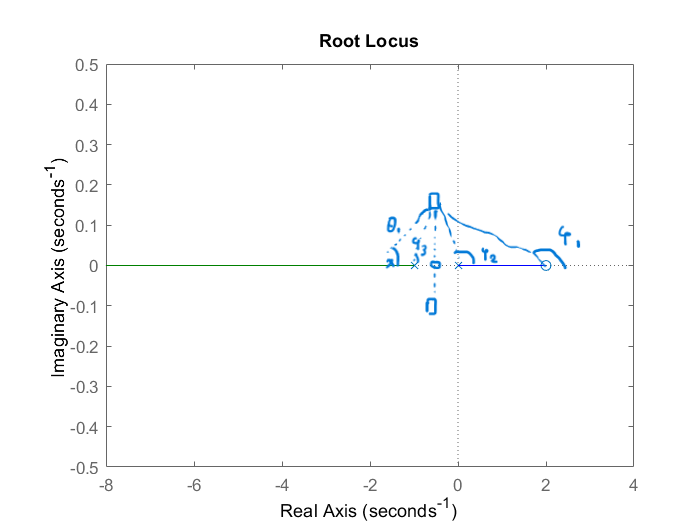
\includegraphics[scale=0.6]{Resources/7.png}
	
	\raggedright
	شرط زاویه : 
	
	\raggedleft
	$-\theta_1 -\phi_3 +90 -\phi_2 +\phi_1 = -180$
	
	$G_c = K\frac{s + 0.3645}{s + 0.33507}$
	
	$K = 0.36$
	
	
\end{problem}


\begin{problem}{سوال هشتم}
	شکل سمت چپ پاسخ پله سیستم بدون کنترلر می باشد. با توجه به قضیه مقدار اولبه می‌انیم که احتمالاً سیستم به فرم ذیل بوده است.
	
	\raggedleft
	$G(s) = \frac{\alpha s^m+...}{s*(\beta s^n + ...)}$
	
	$m = n$
	
	$\underset{s\to \infty }{\mathop{\lim }}\,sG(s)=G(0)$
	
	\raggedright
	شکل سمت راست سیستم با کنترلر را با اورشوت نشان می‌دهد. این به این معناست که کنترلر قطعاً نمی‌توانسته به فرم \lr{lead} یا \lr{lag} باشد. همچنین به فرم \lr{PD} هم نمی باشد چرا که برای حصول به مقدار اولیه صفر مرتبه مخرج باید از مرتبه صورت بزرگتر باشد. 
	
	پس می‌توان نتیجه گرفت که در دینامیک کنترلر مرتبه مخرج بزرگتر از صورت می‌باشد.
	

\end{problem}


\begin{problem}{سوال نهم}
	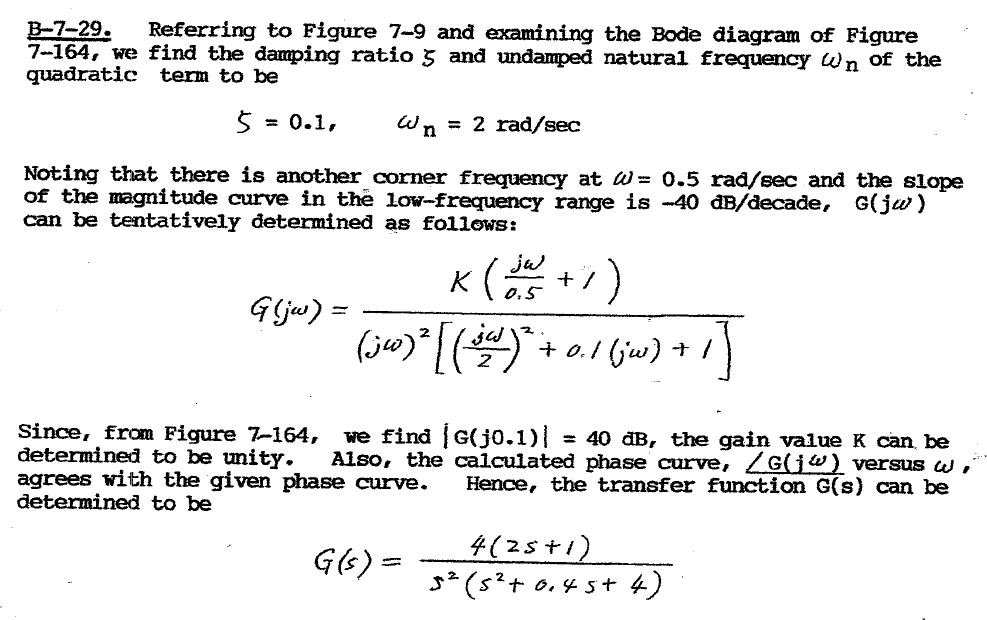
\includegraphics[scale=0.8]{Resources/6.png}
	
	
\end{problem}


\begin{problem}{سوال دهم}
	قطب های مطلوب به فرم زیر بدست می‌آیند.
	
	\raggedleft
	$\zeta = \sqrt{\frac{\ln(PO)^2}{\pi(\ln(PO))^2}} = 0.718$
	
	$t_s = \frac{4}{\zeta \omega_n} => \omega_n = 3.95  $
	
	$s = -\zeta\omega_n \pm j\omega_n\sqrt{1-\zeta^2}$
	
	$s = -2.22 \pm j2.74$
	
	\centering
	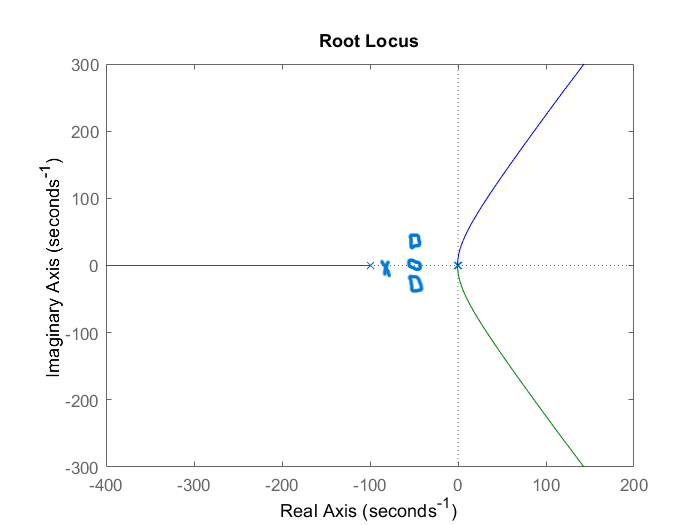
\includegraphics[scale=0.7]{Resources/5.png}
	
	\raggedright
	همانطور که در شکل نشان داده شده است صفر کنترلر را برابر با بخش حقیقی قطب های مطلوب سیستم حلقه بسته انتخاب می‌کنیم حال شرط زاویه را می‌نویسیم.
	
	تعریف :
	\raggedright
	
	$\phi_1$ : زاویه بین قطب -100 
	
	$\phi_2$ : زاویه بین قسمت مثبت محور افقی و -1
	
	$\phi_3$ : زاویه قطب روی 0
	
	$\theta_1$ : زاویه صفر که نود درجه هست
	
	شرط زاویه:
	
	\raggedleft
	$-\phi_1 - \theta_1 + 90 - \phi_2 - \phi_3 = 180$
	
	$-tan^{-1}(\frac{2.74}{97.78}) - \theta_1 + 90 - (180 - tan^{-1}(\frac{2.74}{1.22})) - (180 - tan^{-1}(\frac{2.74}{2.22})) = 180$
	
	$\theta_1 = 24.34$
	
	$G_c = K \frac{s+2.22}{s+8.3}$
	
	$|GG_c(s = -2.22+j2.74)| = 1$
	
	$\frac{100K(2.74)}{\sqrt{2.22^2+2.74^2} \sqrt{1.22^2+2.74^2} \sqrt{97.78^2 + 2.74^2} \sqrt{6.08^2 + 2.74^2}} = 1$
	
	$K = 25.181$
	
	$G_c = 25.181\frac{s+2.22}{s+8.3}$
	
	\raggedright
	می توانید برای اهداف کنترلی یک \lr{prefilter} دلخواه انتخاب کرده و پاسخ را در حضور آن بررسی کنید. این بخش به دلیل دلخواه بودن بر عهده دانشجو قرار داده شده است.
	
\end{problem}


\raggedleft
\section{ بخش تکمیلی (30 نمره)}

\begin{problem}{سوال یازدهم}
	
\end{problem}



\begin{problem}{سوال دوازدهم}
	
\end{problem}



\begin{problem}{سوال سیزدهم}
	برای حل این سوال، ابتدا باید تابع تبدیل سیستم حلقه بسته را با استفاده از تابع تبدیل کنترل‌کننده $( C(s) )$ و تابع تبدیل سیستم $( G(s) )$ بدست آوریم. سپس، با تنظیم مقادیر $( k_p )، ( k_i )، و ( k_d )$ به گونه‌ای که صفرهای مورد نظر را ایجاد کنند، تأثیر آن‌ها را بر روی سیستم بررسی می‌کنیم.
	تابع تبدیل کنترل‌کننده $( C(s) )$ به صورت زیر است:
	
	\raggedleft
	
	$C(s)=kp​+ski​​+kd​s$
	
	\raggedright
	
	و تابع تبدیل سیستم $( G(s) )$ به صورت زیر است:
	
	\raggedleft
	$G(s)=\frac{1}{(s+2)(s+3)}$
	
	\raggedright
	
	تابع تبدیل حلقه بسته $( T(s) )$ با فرض فیدبک واحد به صورت زیر خواهد بود:
	
	\raggedleft
	$T(s)=\frac{C(s)G(s)}{1+C(s)G(s)}$
	
	\raggedright
	
	برای داشتن صفرهای $( z = -3 \pm j )$ در تابع تبدیل حلقه بسته، باید تابع تبدیل کنترل‌کننده $( C(s) )$ را به گونه‌ای تنظیم کنیم که این صفرها را در مخرج تابع تبدیل حلقه بسته ایجاد کند. این کار با افزودن یک جمله به تابع تبدیل کنترل‌کننده که صفرهای مورد نظر را ایجاد می‌کند، امکان‌پذیر است.
	
	به عنوان مثال، اگر یک جمله به صورت $( (s + 3 + j)(s + 3 - j) )$ به مخرج تابع تبدیل کنترل‌کننده اضافه کنیم، صفرهای مورد نظر را خواهیم داشت. این جمله را می‌توان با تنظیم مقادیر $( k_p )،( k_i )، و ( k_d )$ ایجاد کرد.
	
	تغییرات در ضرایب کنترل‌کننده می‌تواند تأثیرات مختلفی بر روی پاسخ سیستم داشته باشد، از جمله تغییر در سرعت پاسخ، میزان ارتعاش، و زمان نشستن سیستم. برای مثال، افزایش $( k_p )$ می‌تواند سرعت پاسخ سیستم را افزایش دهد، در حالی که افزایش $( k_d ) $می‌تواند به کاهش ارتعاشات و بهبود پایداری کمک کند. همچنین، $( k_i )$ برای رفع خطای دائمی در سیستم‌های کنترلی استفاده می‌شود.
	
	برای تحلیل دقیق‌تر و بررسی تأثیرات این تغییرات، می‌توان از روش‌های تحلیلی مانند مکان هندسی ریشه‌ها \lr{(Root Locus) }استفاده کرد. این روش به ما امکان می‌دهد که ببینیم با تغییر ضرایب کنترل‌کننده، قطب‌ها و صفرهای سیستم چگونه در صفحه \lr{s} حرکت می‌کنند و چه تأثیری بر پایداری و پاسخ سیستم دارند.
	
	
\end{problem}


\begin{problem}{سوال چهاردهم}
	در این سوال با توجه به رابطه زیر هرگاه گین 
	\lr{C(s)}
	نسبت به 
	\lr{G(s)}
	بسیار بالاتر باشد در حالت دائم تاثیر اغتشاش حذف می‌شود.
	
	\raggedleft
	$Y(s) = \frac{C(s)G(s)}{1 + C(s)G(s)} R(s) + \frac{G(s)}{1 + C(s)G(s)} D(s)$
	
	\raggedright
	
	برای سیستم های ناپایدار طراحی کنترلر \lr{PID} مناسب تر است.
	می توان نشان داد کنترلر زیر شرایط سوال را برآورده می‌کند.
	
	\raggedleft
	$C(s) = 0.8742 + \frac{1.2239}{s}$

	

	
\end{problem}


\begin{problem}{سوال پانزدهم}
	دقیقاً مانند سوال قبل حل این سوال نیز نیازمند یک کنترلر \lr{PI} می‌باشد.
	البته تنظیم حد فاز با پهنای باند داده شده برای این سیستم امکان پذیر نمی باشد.
	
	$C(s) = 1.414 + \frac{0.02475}{s}$
	
	کنترلر بالا تقریباً شرایط سوال را برآورده می‌کند.
	
\end{problem}


\end{document}
